\documentclass[twoside]{book}

% Packages required by doxygen
\usepackage{calc}
\usepackage{doxygen}
\usepackage{graphicx}
\usepackage[utf8]{inputenc}
\usepackage{makeidx}
\usepackage{multicol}
\usepackage{multirow}
\usepackage{textcomp}
\usepackage[table]{xcolor}

% Font selection
\usepackage[T1]{fontenc}
\usepackage{mathptmx}
\usepackage[scaled=.90]{helvet}
\usepackage{courier}
\usepackage{amssymb}
\usepackage{sectsty}
\renewcommand{\familydefault}{\sfdefault}
\allsectionsfont{%
  \fontseries{bc}\selectfont%
  \color{darkgray}%
}
\renewcommand{\DoxyLabelFont}{%
  \fontseries{bc}\selectfont%
  \color{darkgray}%
}

% Page & text layout
\usepackage{geometry}
\geometry{%
  a4paper,%
  top=2.5cm,%
  bottom=2.5cm,%
  left=2.5cm,%
  right=2.5cm%
}
\tolerance=750
\hfuzz=15pt
\hbadness=750
\setlength{\emergencystretch}{15pt}
\setlength{\parindent}{0cm}
\setlength{\parskip}{0.2cm}
\makeatletter
\renewcommand{\paragraph}{%
  \@startsection{paragraph}{4}{0ex}{-1.0ex}{1.0ex}{%
    \normalfont\normalsize\bfseries\SS@parafont%
  }%
}
\renewcommand{\subparagraph}{%
  \@startsection{subparagraph}{5}{0ex}{-1.0ex}{1.0ex}{%
    \normalfont\normalsize\bfseries\SS@subparafont%
  }%
}
\makeatother

% Headers & footers
\usepackage{fancyhdr}
\pagestyle{fancyplain}
\fancyhead[LE]{\fancyplain{}{\bfseries\thepage}}
\fancyhead[CE]{\fancyplain{}{}}
\fancyhead[RE]{\fancyplain{}{\bfseries\leftmark}}
\fancyhead[LO]{\fancyplain{}{\bfseries\rightmark}}
\fancyhead[CO]{\fancyplain{}{}}
\fancyhead[RO]{\fancyplain{}{\bfseries\thepage}}
\fancyfoot[LE]{\fancyplain{}{}}
\fancyfoot[CE]{\fancyplain{}{}}
\fancyfoot[RE]{\fancyplain{}{\bfseries\scriptsize Generated on Tue Jan 12 2016 19\-:54\-:58 for My Project by Doxygen }}
\fancyfoot[LO]{\fancyplain{}{\bfseries\scriptsize Generated on Tue Jan 12 2016 19\-:54\-:58 for My Project by Doxygen }}
\fancyfoot[CO]{\fancyplain{}{}}
\fancyfoot[RO]{\fancyplain{}{}}
\renewcommand{\footrulewidth}{0.4pt}
\renewcommand{\chaptermark}[1]{%
  \markboth{#1}{}%
}
\renewcommand{\sectionmark}[1]{%
  \markright{\thesection\ #1}%
}

% Indices & bibliography
\usepackage{natbib}
\usepackage[titles]{tocloft}
\setcounter{tocdepth}{3}
\setcounter{secnumdepth}{5}
\makeindex

% Hyperlinks (required, but should be loaded last)
\usepackage{ifpdf}
\ifpdf
  \usepackage[pdftex,pagebackref=true]{hyperref}
\else
  \usepackage[ps2pdf,pagebackref=true]{hyperref}
\fi
\hypersetup{%
  colorlinks=true,%
  linkcolor=blue,%
  citecolor=blue,%
  unicode%
}

% Custom commands
\newcommand{\clearemptydoublepage}{%
  \newpage{\pagestyle{empty}\cleardoublepage}%
}


%===== C O N T E N T S =====

\begin{document}

% Titlepage & ToC
\hypersetup{pageanchor=false}
\pagenumbering{roman}
\begin{titlepage}
\vspace*{7cm}
\begin{center}%
{\Large My Project }\\
\vspace*{1cm}
{\large Generated by Doxygen 1.8.6}\\
\vspace*{0.5cm}
{\small Tue Jan 12 2016 19:54:58}\\
\end{center}
\end{titlepage}
\clearemptydoublepage
\tableofcontents
\clearemptydoublepage
\pagenumbering{arabic}
\hypersetup{pageanchor=true}

%--- Begin generated contents ---
\chapter{Hierarchical Index}
\section{Class Hierarchy}
This inheritance list is sorted roughly, but not completely, alphabetically\-:\begin{DoxyCompactList}
\item \contentsline{section}{Block\-Colours}{\pageref{classBlockColours}}{}
\item \contentsline{section}{Game\-Asset}{\pageref{classGameAsset}}{}
\begin{DoxyCompactList}
\item \contentsline{section}{Cube\-Asset}{\pageref{classCubeAsset}}{}
\item \contentsline{section}{Diamond\-Asset}{\pageref{classDiamondAsset}}{}
\end{DoxyCompactList}
\item \contentsline{section}{Game\-Asset\-Manager}{\pageref{classGameAssetManager}}{}
\item \contentsline{section}{Game\-World}{\pageref{classGameWorld}}{}
\item \contentsline{section}{S\-D\-L\-Window\-Deleter}{\pageref{structSDLWindowDeleter}}{}
\end{DoxyCompactList}

\chapter{Class Index}
\section{Class List}
Here are the classes, structs, unions and interfaces with brief descriptions\-:\begin{DoxyCompactList}
\item\contentsline{section}{\hyperlink{classBlockColours}{Block\-Colours} }{\pageref{classBlockColours}}{}
\item\contentsline{section}{\hyperlink{classCubeAsset}{Cube\-Asset} }{\pageref{classCubeAsset}}{}
\item\contentsline{section}{\hyperlink{classDiamondAsset}{Diamond\-Asset} }{\pageref{classDiamondAsset}}{}
\item\contentsline{section}{\hyperlink{classGameAsset}{Game\-Asset} }{\pageref{classGameAsset}}{}
\item\contentsline{section}{\hyperlink{classGameAssetManager}{Game\-Asset\-Manager} }{\pageref{classGameAssetManager}}{}
\item\contentsline{section}{\hyperlink{classGameWorld}{Game\-World} }{\pageref{classGameWorld}}{}
\item\contentsline{section}{\hyperlink{structSDLWindowDeleter}{S\-D\-L\-Window\-Deleter} }{\pageref{structSDLWindowDeleter}}{}
\end{DoxyCompactList}

\chapter{Class Documentation}
\hypertarget{classBlockColours}{\section{Block\-Colours Class Reference}
\label{classBlockColours}\index{Block\-Colours@{Block\-Colours}}
}
\subsection*{Public Attributes}
\begin{DoxyCompactItemize}
\item 
\hypertarget{classBlockColours_a163b4bcb68e7a8125fa75492d0de0f74}{glm\-::vec3 {\bfseries C\-O\-L\-O\-U\-R\-\_\-\-R\-A\-N\-D\-O\-M} = glm\-::vec3(-\/0.\-1, -\/0.\-1, -\/0.\-1)}\label{classBlockColours_a163b4bcb68e7a8125fa75492d0de0f74}

\item 
\hypertarget{classBlockColours_a6146f2089aa5aed2fc8460d1104d12cb}{glm\-::vec3 {\bfseries C\-O\-L\-O\-U\-R\-\_\-\-R\-E\-D} = glm\-::vec3(255, 0, 0)}\label{classBlockColours_a6146f2089aa5aed2fc8460d1104d12cb}

\item 
\hypertarget{classBlockColours_adf672de5a16ac2b4809eed23ccde6164}{glm\-::vec3 {\bfseries C\-O\-L\-O\-U\-R\-\_\-\-G\-R\-E\-E\-N} = glm\-::vec3(0, 255, 0)}\label{classBlockColours_adf672de5a16ac2b4809eed23ccde6164}

\item 
\hypertarget{classBlockColours_a176ffc07cdacf5f095650e55a8e651fb}{glm\-::vec3 {\bfseries C\-O\-L\-O\-U\-R\-\_\-\-B\-L\-U\-E} = glm\-::vec3(0, 0, 255)}\label{classBlockColours_a176ffc07cdacf5f095650e55a8e651fb}

\item 
\hypertarget{classBlockColours_a391d047f40a0b6eb496b2795d46cb963}{glm\-::vec3 {\bfseries C\-O\-L\-O\-U\-R\-\_\-\-N\-O\-N\-E} = glm\-::vec3(0, 0, 0)}\label{classBlockColours_a391d047f40a0b6eb496b2795d46cb963}

\end{DoxyCompactItemize}


The documentation for this class was generated from the following file\-:\begin{DoxyCompactItemize}
\item 
Block\-Colours.\-h\end{DoxyCompactItemize}

\hypertarget{classCubeAsset}{\section{Cube\-Asset Class Reference}
\label{classCubeAsset}\index{Cube\-Asset@{Cube\-Asset}}
}
Inheritance diagram for Cube\-Asset\-:\begin{figure}[H]
\begin{center}
\leavevmode
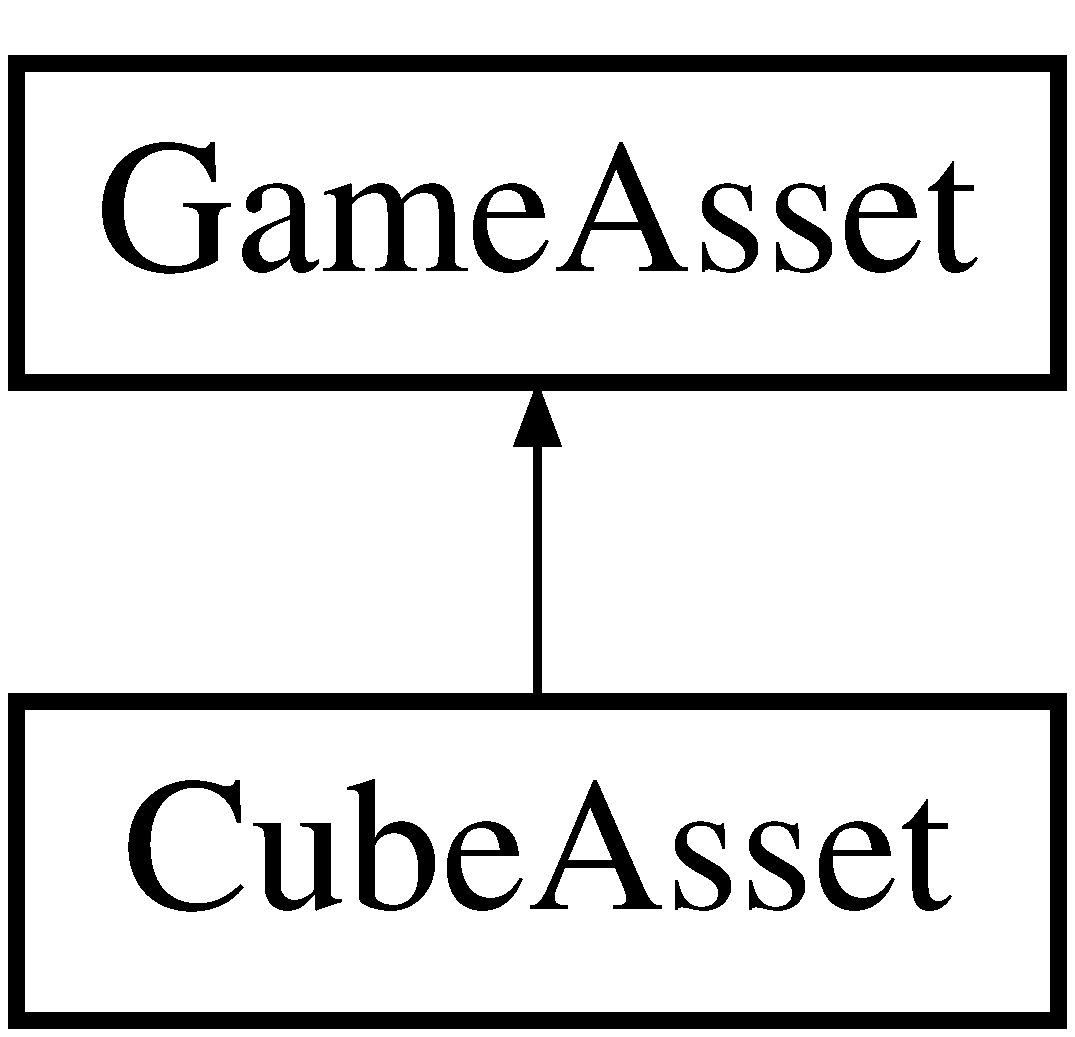
\includegraphics[height=2.000000cm]{classCubeAsset}
\end{center}
\end{figure}
\subsection*{Public Member Functions}
\begin{DoxyCompactItemize}
\item 
\hyperlink{classCubeAsset_a94f08a414e5b04ad37acffa3c1a1259b}{Cube\-Asset} (glm\-::vec3, glm\-::vec3)
\item 
\hypertarget{classCubeAsset_a1af568486056e254ffcf98fd99947bfe}{virtual void {\bfseries Draw} (G\-Luint)}\label{classCubeAsset_a1af568486056e254ffcf98fd99947bfe}

\item 
\hypertarget{classCubeAsset_a7198b512f3dfc44d40c82f6025dc3156}{float {\bfseries rf} ()}\label{classCubeAsset_a7198b512f3dfc44d40c82f6025dc3156}

\item 
glm\-::vec3 \hyperlink{classCubeAsset_a4cfa6bb819ac03a9c85cf0ae979704b7}{Get\-Vec3} ()
\end{DoxyCompactItemize}


\subsection{Constructor \& Destructor Documentation}
\hypertarget{classCubeAsset_a94f08a414e5b04ad37acffa3c1a1259b}{\index{Cube\-Asset@{Cube\-Asset}!Cube\-Asset@{Cube\-Asset}}
\index{Cube\-Asset@{Cube\-Asset}!CubeAsset@{Cube\-Asset}}
\subsubsection[{Cube\-Asset}]{\setlength{\rightskip}{0pt plus 5cm}Cube\-Asset\-::\-Cube\-Asset (
\begin{DoxyParamCaption}
\item[{glm\-::vec3}]{p, }
\item[{glm\-::vec3}]{c}
\end{DoxyParamCaption}
)}}\label{classCubeAsset_a94f08a414e5b04ad37acffa3c1a1259b}
Transfer buffers to the G\-P\-U create buffer immediately bind the buffer and transfer the data

\subsection{Member Function Documentation}
\hypertarget{classCubeAsset_a4cfa6bb819ac03a9c85cf0ae979704b7}{\index{Cube\-Asset@{Cube\-Asset}!Get\-Vec3@{Get\-Vec3}}
\index{Get\-Vec3@{Get\-Vec3}!CubeAsset@{Cube\-Asset}}
\subsubsection[{Get\-Vec3}]{\setlength{\rightskip}{0pt plus 5cm}glm\-::vec3 Cube\-Asset\-::\-Get\-Vec3 (
\begin{DoxyParamCaption}
{}
\end{DoxyParamCaption}
)}}\label{classCubeAsset_a4cfa6bb819ac03a9c85cf0ae979704b7}
Returns the vec3 of the cube 

The documentation for this class was generated from the following files\-:\begin{DoxyCompactItemize}
\item 
Cube\-Asset.\-h\item 
Cube\-Asset.\-cc\end{DoxyCompactItemize}

\hypertarget{classDiamondAsset}{\section{Diamond\-Asset Class Reference}
\label{classDiamondAsset}\index{Diamond\-Asset@{Diamond\-Asset}}
}
Inheritance diagram for Diamond\-Asset\-:\begin{figure}[H]
\begin{center}
\leavevmode
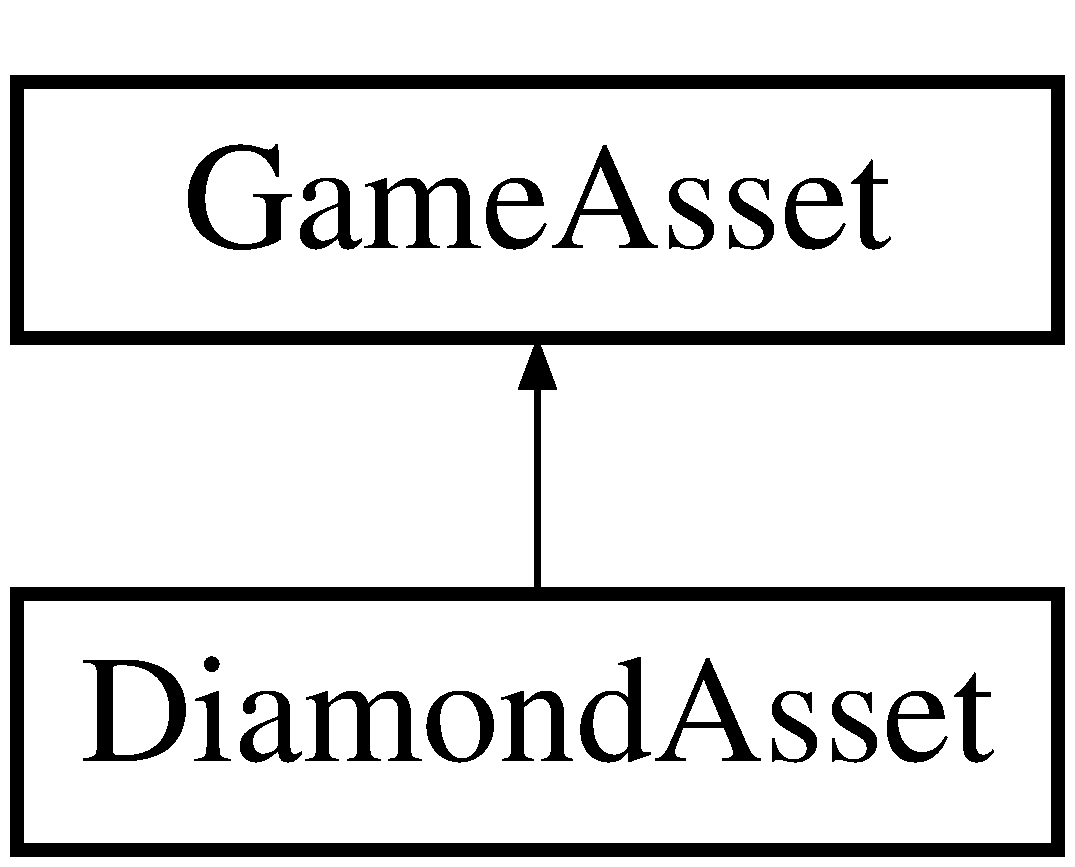
\includegraphics[height=2.000000cm]{classDiamondAsset}
\end{center}
\end{figure}
\subsection*{Public Member Functions}
\begin{DoxyCompactItemize}
\item 
\hyperlink{classDiamondAsset_af17cd961010d8b40199f8fe3b8dc1912}{Diamond\-Asset} (glm\-::vec3, glm\-::vec3)
\item 
\hypertarget{classDiamondAsset_a0c259031894623285b3b511321c73abb}{virtual void {\bfseries Draw} (G\-Luint)}\label{classDiamondAsset_a0c259031894623285b3b511321c73abb}

\item 
\hypertarget{classDiamondAsset_ac6a40e3db3fe79301c47c7645a8078fa}{float {\bfseries rf} ()}\label{classDiamondAsset_ac6a40e3db3fe79301c47c7645a8078fa}

\item 
glm\-::vec3 \hyperlink{classDiamondAsset_aba645e9943cfb411184bf33e4f27e168}{Get\-Vec3} ()
\end{DoxyCompactItemize}


\subsection{Constructor \& Destructor Documentation}
\hypertarget{classDiamondAsset_af17cd961010d8b40199f8fe3b8dc1912}{\index{Diamond\-Asset@{Diamond\-Asset}!Diamond\-Asset@{Diamond\-Asset}}
\index{Diamond\-Asset@{Diamond\-Asset}!DiamondAsset@{Diamond\-Asset}}
\subsubsection[{Diamond\-Asset}]{\setlength{\rightskip}{0pt plus 5cm}Diamond\-Asset\-::\-Diamond\-Asset (
\begin{DoxyParamCaption}
\item[{glm\-::vec3}]{p, }
\item[{glm\-::vec3}]{c}
\end{DoxyParamCaption}
)}}\label{classDiamondAsset_af17cd961010d8b40199f8fe3b8dc1912}
Transfer buffers to the G\-P\-U create buffer immediately bind the buffer and transfer the data

\subsection{Member Function Documentation}
\hypertarget{classDiamondAsset_aba645e9943cfb411184bf33e4f27e168}{\index{Diamond\-Asset@{Diamond\-Asset}!Get\-Vec3@{Get\-Vec3}}
\index{Get\-Vec3@{Get\-Vec3}!DiamondAsset@{Diamond\-Asset}}
\subsubsection[{Get\-Vec3}]{\setlength{\rightskip}{0pt plus 5cm}glm\-::vec3 Diamond\-Asset\-::\-Get\-Vec3 (
\begin{DoxyParamCaption}
{}
\end{DoxyParamCaption}
)}}\label{classDiamondAsset_aba645e9943cfb411184bf33e4f27e168}
Returns the vec3 of the cube 

The documentation for this class was generated from the following files\-:\begin{DoxyCompactItemize}
\item 
Diamond\-Asset.\-h\item 
Diamond\-Asset.\-cc\end{DoxyCompactItemize}

\hypertarget{classGameAsset}{\section{Game\-Asset Class Reference}
\label{classGameAsset}\index{Game\-Asset@{Game\-Asset}}
}
Inheritance diagram for Game\-Asset\-:\begin{figure}[H]
\begin{center}
\leavevmode
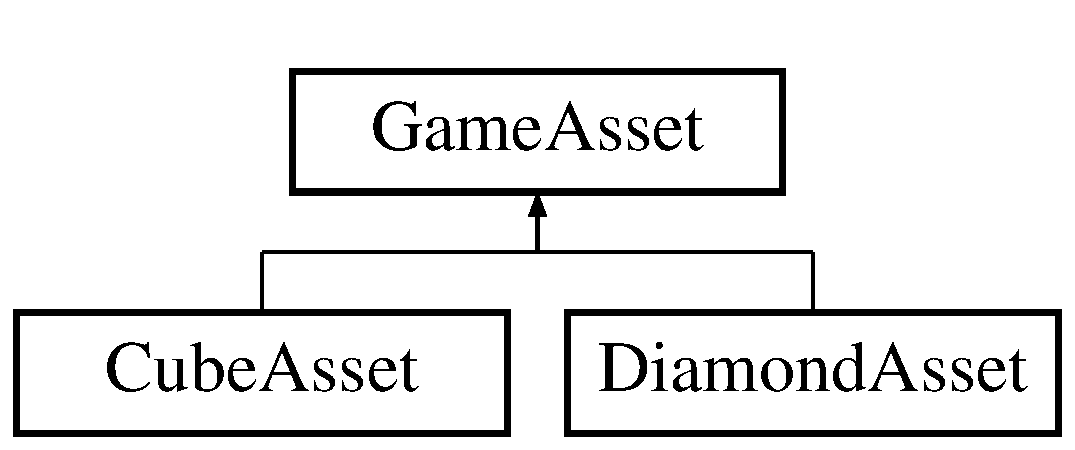
\includegraphics[height=2.000000cm]{classGameAsset}
\end{center}
\end{figure}
\subsection*{Public Member Functions}
\begin{DoxyCompactItemize}
\item 
\hypertarget{classGameAsset_a961aa51ca0a9961fc584c0b5d5431300}{virtual void {\bfseries Draw} (G\-Luint)=0}\label{classGameAsset_a961aa51ca0a9961fc584c0b5d5431300}

\end{DoxyCompactItemize}


The documentation for this class was generated from the following file\-:\begin{DoxyCompactItemize}
\item 
Game\-Asset.\-h\end{DoxyCompactItemize}

\hypertarget{classGameAssetManager}{\section{Game\-Asset\-Manager Class Reference}
\label{classGameAssetManager}\index{Game\-Asset\-Manager@{Game\-Asset\-Manager}}
}


{\ttfamily \#include $<$Game\-Asset\-Manager.\-h$>$}

\subsection*{Public Member Functions}
\begin{DoxyCompactItemize}
\item 
\hyperlink{classGameAssetManager_aaa0d58e276cc10ad91a7457085598a71}{Game\-Asset\-Manager} (Application\-Mode)
\item 
virtual \hyperlink{classGameAssetManager_a1270bd61ecbcca563f079803e40c9b77}{$\sim$\-Game\-Asset\-Manager} ()
\item 
\hyperlink{classGameAssetManager_a2c9adcb72faa154c87eadc9bafe5269d}{Game\-Asset\-Manager} (\hyperlink{classGameAssetManager}{Game\-Asset\-Manager} const \&)
\item 
\hyperlink{classGameAssetManager_a44f6e2fd6b8ff1dd64e5697f1be7386d}{Game\-Asset\-Manager} (\hyperlink{classGameAssetManager}{Game\-Asset\-Manager} const \&\&)
\item 
void \hyperlink{classGameAssetManager_ac72678a4ad5378c685aa6bae84a4e712}{operator=} (\hyperlink{classGameAssetManager}{Game\-Asset\-Manager} const \&)
\item 
void \hyperlink{classGameAssetManager_a72921fb5f6501cbef808756b9da1a777}{Add\-Asset} (std\-::shared\-\_\-ptr$<$ \hyperlink{classCubeAsset}{Cube\-Asset} $>$)
\item 
void \hyperlink{classGameAssetManager_a01605355f3a62fcda0b3c1f006d4c7e6}{Add\-Asset\-Diamond} (std\-::shared\-\_\-ptr$<$ \hyperlink{classGameAsset}{Game\-Asset} $>$)
\item 
void \hyperlink{classGameAssetManager_ab4f0a7ef366adcdb87794c4a3a656d8c}{Remove\-Asset} (glm\-::vec3, glm\-::vec3)
\item 
void \hyperlink{classGameAssetManager_a1f42ae294d29e0f0f0730686a3e306e3}{Remove\-All} ()
\item 
void \hyperlink{classGameAssetManager_a1c4c7e39bdc8aac2864fcdf4c5ec4c5b}{Draw} (glm\-::mat4, glm\-::mat4)
\item 
std\-::vector$<$ std\-::shared\-\_\-ptr\\*
$<$ \hyperlink{classCubeAsset}{Cube\-Asset} $>$ $>$ \hyperlink{classGameAssetManager_a0ce5254413ecd200a19410f756a10ce9}{Get\-Assets} ()
\end{DoxyCompactItemize}


\subsection{Detailed Description}
\hyperlink{classGameAssetManager}{Game\-Asset\-Manager} is a container for Game\-Assets. It also provides utility functions to to create a simple Open\-G\-L program that can be used to draw a simple \hyperlink{classGameAsset}{Game\-Asset}. 

\subsection{Constructor \& Destructor Documentation}
\hypertarget{classGameAssetManager_aaa0d58e276cc10ad91a7457085598a71}{\index{Game\-Asset\-Manager@{Game\-Asset\-Manager}!Game\-Asset\-Manager@{Game\-Asset\-Manager}}
\index{Game\-Asset\-Manager@{Game\-Asset\-Manager}!GameAssetManager@{Game\-Asset\-Manager}}
\subsubsection[{Game\-Asset\-Manager}]{\setlength{\rightskip}{0pt plus 5cm}Game\-Asset\-Manager\-::\-Game\-Asset\-Manager (
\begin{DoxyParamCaption}
\item[{Application\-Mode}]{mode}
\end{DoxyParamCaption}
)\hspace{0.3cm}{\ttfamily [explicit]}}}\label{classGameAssetManager_aaa0d58e276cc10ad91a7457085598a71}
Creates a \hyperlink{classGameAssetManager}{Game\-Asset\-Manager} to load the correct shaders based on the Application\-Mode. \hypertarget{classGameAssetManager_a1270bd61ecbcca563f079803e40c9b77}{\index{Game\-Asset\-Manager@{Game\-Asset\-Manager}!$\sim$\-Game\-Asset\-Manager@{$\sim$\-Game\-Asset\-Manager}}
\index{$\sim$\-Game\-Asset\-Manager@{$\sim$\-Game\-Asset\-Manager}!GameAssetManager@{Game\-Asset\-Manager}}
\subsubsection[{$\sim$\-Game\-Asset\-Manager}]{\setlength{\rightskip}{0pt plus 5cm}Game\-Asset\-Manager\-::$\sim$\-Game\-Asset\-Manager (
\begin{DoxyParamCaption}
{}
\end{DoxyParamCaption}
)\hspace{0.3cm}{\ttfamily [virtual]}}}\label{classGameAssetManager_a1270bd61ecbcca563f079803e40c9b77}
Deletes a \hyperlink{classGameAssetManager}{Game\-Asset\-Manager}, in particular it will clean up any modifications to the Open\-G\-L state. \hypertarget{classGameAssetManager_a2c9adcb72faa154c87eadc9bafe5269d}{\index{Game\-Asset\-Manager@{Game\-Asset\-Manager}!Game\-Asset\-Manager@{Game\-Asset\-Manager}}
\index{Game\-Asset\-Manager@{Game\-Asset\-Manager}!GameAssetManager@{Game\-Asset\-Manager}}
\subsubsection[{Game\-Asset\-Manager}]{\setlength{\rightskip}{0pt plus 5cm}Game\-Asset\-Manager\-::\-Game\-Asset\-Manager (
\begin{DoxyParamCaption}
\item[{{\bf Game\-Asset\-Manager} const \&}]{the\-\_\-manager}
\end{DoxyParamCaption}
)}}\label{classGameAssetManager_a2c9adcb72faa154c87eadc9bafe5269d}
Unimplemented copy constructor -- this means that the \hyperlink{classGameAssetManager}{Game\-Asset\-Manager} may not work as you'd expect when being copied. \hypertarget{classGameAssetManager_a44f6e2fd6b8ff1dd64e5697f1be7386d}{\index{Game\-Asset\-Manager@{Game\-Asset\-Manager}!Game\-Asset\-Manager@{Game\-Asset\-Manager}}
\index{Game\-Asset\-Manager@{Game\-Asset\-Manager}!GameAssetManager@{Game\-Asset\-Manager}}
\subsubsection[{Game\-Asset\-Manager}]{\setlength{\rightskip}{0pt plus 5cm}Game\-Asset\-Manager\-::\-Game\-Asset\-Manager (
\begin{DoxyParamCaption}
\item[{{\bf Game\-Asset\-Manager} const \&\&}]{the\-\_\-manager}
\end{DoxyParamCaption}
)}}\label{classGameAssetManager_a44f6e2fd6b8ff1dd64e5697f1be7386d}
Unimplemented move constructor -- this unimplemented method violates the C++11 move semantics for \hyperlink{classGameAssetManager}{Game\-Asset\-Manager}. 

\subsection{Member Function Documentation}
\hypertarget{classGameAssetManager_a72921fb5f6501cbef808756b9da1a777}{\index{Game\-Asset\-Manager@{Game\-Asset\-Manager}!Add\-Asset@{Add\-Asset}}
\index{Add\-Asset@{Add\-Asset}!GameAssetManager@{Game\-Asset\-Manager}}
\subsubsection[{Add\-Asset}]{\setlength{\rightskip}{0pt plus 5cm}void Game\-Asset\-Manager\-::\-Add\-Asset (
\begin{DoxyParamCaption}
\item[{std\-::shared\-\_\-ptr$<$ {\bf Cube\-Asset} $>$}]{cube\-\_\-asset}
\end{DoxyParamCaption}
)}}\label{classGameAssetManager_a72921fb5f6501cbef808756b9da1a777}
Adds a \hyperlink{classGameAsset}{Game\-Asset} to the scene graph. \hypertarget{classGameAssetManager_a01605355f3a62fcda0b3c1f006d4c7e6}{\index{Game\-Asset\-Manager@{Game\-Asset\-Manager}!Add\-Asset\-Diamond@{Add\-Asset\-Diamond}}
\index{Add\-Asset\-Diamond@{Add\-Asset\-Diamond}!GameAssetManager@{Game\-Asset\-Manager}}
\subsubsection[{Add\-Asset\-Diamond}]{\setlength{\rightskip}{0pt plus 5cm}void Game\-Asset\-Manager\-::\-Add\-Asset\-Diamond (
\begin{DoxyParamCaption}
\item[{std\-::shared\-\_\-ptr$<$ {\bf Game\-Asset} $>$}]{diamond\-\_\-asset}
\end{DoxyParamCaption}
)}}\label{classGameAssetManager_a01605355f3a62fcda0b3c1f006d4c7e6}
Adds a \hyperlink{classGameAsset}{Game\-Asset} to the scene graph. T\-H\-I\-S A\-D\-D\-S A D\-I\-A\-M\-O\-N\-D A\-S\-S\-E\-T, B\-U\-T D\-O\-E\-S N\-O\-T G\-I\-V\-E I\-T T\-H\-E S\-A\-M\-E F\-U\-N\-C\-T\-I\-O\-N\-A\-L\-I\-T\-Y A\-S C\-U\-B\-E\-A\-S\-S\-E\-T \hypertarget{classGameAssetManager_a1c4c7e39bdc8aac2864fcdf4c5ec4c5b}{\index{Game\-Asset\-Manager@{Game\-Asset\-Manager}!Draw@{Draw}}
\index{Draw@{Draw}!GameAssetManager@{Game\-Asset\-Manager}}
\subsubsection[{Draw}]{\setlength{\rightskip}{0pt plus 5cm}void Game\-Asset\-Manager\-::\-Draw (
\begin{DoxyParamCaption}
\item[{glm\-::mat4}]{cam\-\_\-proj, }
\item[{glm\-::mat4}]{cam\-\_\-view}
\end{DoxyParamCaption}
)}}\label{classGameAssetManager_a1c4c7e39bdc8aac2864fcdf4c5ec4c5b}
Draws each \hyperlink{classGameAsset}{Game\-Asset} in the scene graph. \hypertarget{classGameAssetManager_a0ce5254413ecd200a19410f756a10ce9}{\index{Game\-Asset\-Manager@{Game\-Asset\-Manager}!Get\-Assets@{Get\-Assets}}
\index{Get\-Assets@{Get\-Assets}!GameAssetManager@{Game\-Asset\-Manager}}
\subsubsection[{Get\-Assets}]{\setlength{\rightskip}{0pt plus 5cm}std\-::vector$<$ std\-::shared\-\_\-ptr$<$ {\bf Cube\-Asset} $>$ $>$ Game\-Asset\-Manager\-::\-Get\-Assets (
\begin{DoxyParamCaption}
{}
\end{DoxyParamCaption}
)}}\label{classGameAssetManager_a0ce5254413ecd200a19410f756a10ce9}
Gets the asset list \hypertarget{classGameAssetManager_ac72678a4ad5378c685aa6bae84a4e712}{\index{Game\-Asset\-Manager@{Game\-Asset\-Manager}!operator=@{operator=}}
\index{operator=@{operator=}!GameAssetManager@{Game\-Asset\-Manager}}
\subsubsection[{operator=}]{\setlength{\rightskip}{0pt plus 5cm}void Game\-Asset\-Manager\-::operator= (
\begin{DoxyParamCaption}
\item[{{\bf Game\-Asset\-Manager} const \&}]{the\-\_\-manager}
\end{DoxyParamCaption}
)}}\label{classGameAssetManager_ac72678a4ad5378c685aa6bae84a4e712}
Unimplemented assisgnment operator -- violates the expected semantics for assignment in C++11. \hypertarget{classGameAssetManager_a1f42ae294d29e0f0f0730686a3e306e3}{\index{Game\-Asset\-Manager@{Game\-Asset\-Manager}!Remove\-All@{Remove\-All}}
\index{Remove\-All@{Remove\-All}!GameAssetManager@{Game\-Asset\-Manager}}
\subsubsection[{Remove\-All}]{\setlength{\rightskip}{0pt plus 5cm}void Game\-Asset\-Manager\-::\-Remove\-All (
\begin{DoxyParamCaption}
{}
\end{DoxyParamCaption}
)}}\label{classGameAssetManager_a1f42ae294d29e0f0f0730686a3e306e3}
Removes all of the assets from the world \hypertarget{classGameAssetManager_ab4f0a7ef366adcdb87794c4a3a656d8c}{\index{Game\-Asset\-Manager@{Game\-Asset\-Manager}!Remove\-Asset@{Remove\-Asset}}
\index{Remove\-Asset@{Remove\-Asset}!GameAssetManager@{Game\-Asset\-Manager}}
\subsubsection[{Remove\-Asset}]{\setlength{\rightskip}{0pt plus 5cm}void Game\-Asset\-Manager\-::\-Remove\-Asset (
\begin{DoxyParamCaption}
\item[{glm\-::vec3}]{position, }
\item[{glm\-::vec3}]{offset\-\_\-pos}
\end{DoxyParamCaption}
)}}\label{classGameAssetManager_ab4f0a7ef366adcdb87794c4a3a656d8c}
Removes an asset from the gameworld 

The documentation for this class was generated from the following files\-:\begin{DoxyCompactItemize}
\item 
Game\-Asset\-Manager.\-h\item 
Game\-Asset\-Manager.\-cc\end{DoxyCompactItemize}

\hypertarget{classGameWorld}{\section{Game\-World Class Reference}
\label{classGameWorld}\index{Game\-World@{Game\-World}}
}


{\ttfamily \#include $<$Game\-World.\-h$>$}

\subsection*{Public Member Functions}
\begin{DoxyCompactItemize}
\item 
\hyperlink{classGameWorld_a17a84e57a80600961088afc753036f89}{Game\-World} (Application\-Mode)
\item 
void \hyperlink{classGameWorld_a275418607d8286979b276f165ad5876b}{Draw} ()
\item 
void \hyperlink{classGameWorld_a868f6c145f31f990974b324685f63448}{Camera\-Controller} (int)
\item 
void \hyperlink{classGameWorld_a46e48d65ed762acad6ad9ef40e6c9610}{Move\-Camera} (glm\-::vec2, glm\-::vec2)
\item 
void \hyperlink{classGameWorld_ae029ce82ab27a6bb1b2a1784ddaddaad}{Do\-Action} (int)
\item 
void \hyperlink{classGameWorld_a281a531082e7fcdfde3339445e0e4b22}{Update\-Facing\-Direction} ()
\item 
void \hyperlink{classGameWorld_ab408a83dde217403691c88f8bc498fc1}{Create\-Shape} (std\-::string, int)
\item 
void \hyperlink{classGameWorld_aaa1b24d4bba8b9a9a663b1a809552044}{Change\-Block\-Dist} (int)
\item 
void \hyperlink{classGameWorld_aaaf6174a524d23a4759b15d981304711}{Load\-Map} (std\-::string)
\item 
void \hyperlink{classGameWorld_a00e989074bc585786af91119b0996828}{Set\-Block\-Type} (int)
\item 
bool \hyperlink{classGameWorld_a800d763be7f2980d1eb7f2715616ab97}{Check\-Collision} (glm\-::vec3)
\item 
glm\-::vec3 \hyperlink{classGameWorld_a76ff889cffc8450d74e7ddedda2af7e9}{Get\-Offset} ()
\end{DoxyCompactItemize}
\subsection*{Public Attributes}
\begin{DoxyCompactItemize}
\item 
\hypertarget{classGameWorld_a08474ddb5c961a526ca3a915665459f5}{\hyperlink{classBlockColours}{Block\-Colours} {\bfseries colour\-\_\-manager}}\label{classGameWorld_a08474ddb5c961a526ca3a915665459f5}

\end{DoxyCompactItemize}


\subsection{Detailed Description}
\hyperlink{classGameWorld}{Game\-World} allows us to separate the management of the game world from the nuts and bolts of game loop initialisation. The \hyperlink{classGameWorld}{Game\-World} currently has a very simplified scene graph consisiting of a single \hyperlink{classGameAssetManager}{Game\-Asset\-Manager}. 

\subsection{Constructor \& Destructor Documentation}
\hypertarget{classGameWorld_a17a84e57a80600961088afc753036f89}{\index{Game\-World@{Game\-World}!Game\-World@{Game\-World}}
\index{Game\-World@{Game\-World}!GameWorld@{Game\-World}}
\subsubsection[{Game\-World}]{\setlength{\rightskip}{0pt plus 5cm}Game\-World\-::\-Game\-World (
\begin{DoxyParamCaption}
\item[{Application\-Mode}]{mode}
\end{DoxyParamCaption}
)}}\label{classGameWorld_a17a84e57a80600961088afc753036f89}
We thread the Application\-Mode through the \hyperlink{classGameWorld}{Game\-World} ss we want to read it in from the user. Threading the state through the various function calls is preferable (in this case) to having some kind of global state. 

\subsection{Member Function Documentation}
\hypertarget{classGameWorld_a868f6c145f31f990974b324685f63448}{\index{Game\-World@{Game\-World}!Camera\-Controller@{Camera\-Controller}}
\index{Camera\-Controller@{Camera\-Controller}!GameWorld@{Game\-World}}
\subsubsection[{Camera\-Controller}]{\setlength{\rightskip}{0pt plus 5cm}void Game\-World\-::\-Camera\-Controller (
\begin{DoxyParamCaption}
\item[{int}]{k}
\end{DoxyParamCaption}
)}}\label{classGameWorld_a868f6c145f31f990974b324685f63448}
Handles the keyboard inputs passed from main. \hypertarget{classGameWorld_aaa1b24d4bba8b9a9a663b1a809552044}{\index{Game\-World@{Game\-World}!Change\-Block\-Dist@{Change\-Block\-Dist}}
\index{Change\-Block\-Dist@{Change\-Block\-Dist}!GameWorld@{Game\-World}}
\subsubsection[{Change\-Block\-Dist}]{\setlength{\rightskip}{0pt plus 5cm}void Game\-World\-::\-Change\-Block\-Dist (
\begin{DoxyParamCaption}
\item[{int}]{i}
\end{DoxyParamCaption}
)}}\label{classGameWorld_aaa1b24d4bba8b9a9a663b1a809552044}
Changes block distance \hypertarget{classGameWorld_a800d763be7f2980d1eb7f2715616ab97}{\index{Game\-World@{Game\-World}!Check\-Collision@{Check\-Collision}}
\index{Check\-Collision@{Check\-Collision}!GameWorld@{Game\-World}}
\subsubsection[{Check\-Collision}]{\setlength{\rightskip}{0pt plus 5cm}bool Game\-World\-::\-Check\-Collision (
\begin{DoxyParamCaption}
\item[{glm\-::vec3}]{point}
\end{DoxyParamCaption}
)}}\label{classGameWorld_a800d763be7f2980d1eb7f2715616ab97}
Returns true if the position passed is already filled with a block \hypertarget{classGameWorld_ab408a83dde217403691c88f8bc498fc1}{\index{Game\-World@{Game\-World}!Create\-Shape@{Create\-Shape}}
\index{Create\-Shape@{Create\-Shape}!GameWorld@{Game\-World}}
\subsubsection[{Create\-Shape}]{\setlength{\rightskip}{0pt plus 5cm}void Game\-World\-::\-Create\-Shape (
\begin{DoxyParamCaption}
\item[{std\-::string}]{shape, }
\item[{int}]{size}
\end{DoxyParamCaption}
)}}\label{classGameWorld_ab408a83dde217403691c88f8bc498fc1}
Generates a shape \hypertarget{classGameWorld_ae029ce82ab27a6bb1b2a1784ddaddaad}{\index{Game\-World@{Game\-World}!Do\-Action@{Do\-Action}}
\index{Do\-Action@{Do\-Action}!GameWorld@{Game\-World}}
\subsubsection[{Do\-Action}]{\setlength{\rightskip}{0pt plus 5cm}void Game\-World\-::\-Do\-Action (
\begin{DoxyParamCaption}
\item[{int}]{a}
\end{DoxyParamCaption}
)}}\label{classGameWorld_ae029ce82ab27a6bb1b2a1784ddaddaad}
Handles action codes passed from main \hypertarget{classGameWorld_a275418607d8286979b276f165ad5876b}{\index{Game\-World@{Game\-World}!Draw@{Draw}}
\index{Draw@{Draw}!GameWorld@{Game\-World}}
\subsubsection[{Draw}]{\setlength{\rightskip}{0pt plus 5cm}void Game\-World\-::\-Draw (
\begin{DoxyParamCaption}
{}
\end{DoxyParamCaption}
)}}\label{classGameWorld_a275418607d8286979b276f165ad5876b}
Handles drawing of the camera and game world assets \hypertarget{classGameWorld_a76ff889cffc8450d74e7ddedda2af7e9}{\index{Game\-World@{Game\-World}!Get\-Offset@{Get\-Offset}}
\index{Get\-Offset@{Get\-Offset}!GameWorld@{Game\-World}}
\subsubsection[{Get\-Offset}]{\setlength{\rightskip}{0pt plus 5cm}glm\-::vec3 Game\-World\-::\-Get\-Offset (
\begin{DoxyParamCaption}
{}
\end{DoxyParamCaption}
)}}\label{classGameWorld_a76ff889cffc8450d74e7ddedda2af7e9}
Returns an offset for the space in front of the camera and also calculates block placement based on the camera angle \hypertarget{classGameWorld_aaaf6174a524d23a4759b15d981304711}{\index{Game\-World@{Game\-World}!Load\-Map@{Load\-Map}}
\index{Load\-Map@{Load\-Map}!GameWorld@{Game\-World}}
\subsubsection[{Load\-Map}]{\setlength{\rightskip}{0pt plus 5cm}void Game\-World\-::\-Load\-Map (
\begin{DoxyParamCaption}
\item[{std\-::string}]{filename}
\end{DoxyParamCaption}
)}}\label{classGameWorld_aaaf6174a524d23a4759b15d981304711}
A very bad example of rendering heightmaps Takes in a P\-P\-M file, reads the headers and then the map data \hypertarget{classGameWorld_a46e48d65ed762acad6ad9ef40e6c9610}{\index{Game\-World@{Game\-World}!Move\-Camera@{Move\-Camera}}
\index{Move\-Camera@{Move\-Camera}!GameWorld@{Game\-World}}
\subsubsection[{Move\-Camera}]{\setlength{\rightskip}{0pt plus 5cm}void Game\-World\-::\-Move\-Camera (
\begin{DoxyParamCaption}
\item[{glm\-::vec2}]{motion, }
\item[{glm\-::vec2}]{display}
\end{DoxyParamCaption}
)}}\label{classGameWorld_a46e48d65ed762acad6ad9ef40e6c9610}
Handles the mouse input for the camera \hypertarget{classGameWorld_a00e989074bc585786af91119b0996828}{\index{Game\-World@{Game\-World}!Set\-Block\-Type@{Set\-Block\-Type}}
\index{Set\-Block\-Type@{Set\-Block\-Type}!GameWorld@{Game\-World}}
\subsubsection[{Set\-Block\-Type}]{\setlength{\rightskip}{0pt plus 5cm}void Game\-World\-::\-Set\-Block\-Type (
\begin{DoxyParamCaption}
\item[{int}]{b}
\end{DoxyParamCaption}
)}}\label{classGameWorld_a00e989074bc585786af91119b0996828}
Sets the block type to place \hypertarget{classGameWorld_a281a531082e7fcdfde3339445e0e4b22}{\index{Game\-World@{Game\-World}!Update\-Facing\-Direction@{Update\-Facing\-Direction}}
\index{Update\-Facing\-Direction@{Update\-Facing\-Direction}!GameWorld@{Game\-World}}
\subsubsection[{Update\-Facing\-Direction}]{\setlength{\rightskip}{0pt plus 5cm}void Game\-World\-::\-Update\-Facing\-Direction (
\begin{DoxyParamCaption}
{}
\end{DoxyParamCaption}
)}}\label{classGameWorld_a281a531082e7fcdfde3339445e0e4b22}
Calculates the camera facing direction 

The documentation for this class was generated from the following files\-:\begin{DoxyCompactItemize}
\item 
Game\-World.\-h\item 
Game\-World.\-cc\end{DoxyCompactItemize}

\hypertarget{structSDLWindowDeleter}{\section{S\-D\-L\-Window\-Deleter Struct Reference}
\label{structSDLWindowDeleter}\index{S\-D\-L\-Window\-Deleter@{S\-D\-L\-Window\-Deleter}}
}
\subsection*{Public Member Functions}
\begin{DoxyCompactItemize}
\item 
\hypertarget{structSDLWindowDeleter_a2aedcc99c3756ae090c38badabeb10b1}{void {\bfseries operator()} (S\-D\-L\-\_\-\-Window $\ast$window)}\label{structSDLWindowDeleter_a2aedcc99c3756ae090c38badabeb10b1}

\end{DoxyCompactItemize}


The documentation for this struct was generated from the following file\-:\begin{DoxyCompactItemize}
\item 
main.\-cc\end{DoxyCompactItemize}

%--- End generated contents ---

% Index
\newpage
\phantomsection
\addcontentsline{toc}{chapter}{Index}
\printindex

\end{document}
